% Marco Teorico.
\chapter{Marco te'orico} \label{chap:ssimilar}

\vspace{5 mm}

\section{Data Clustering} \label{sect:dclust}

\subsection{Introducci\'on} \label{sect:dclusti}

Data clustering (o s\'olo clustering), tambien llamado an\'alisis de clusters, an\'alisis de segmentaci\'on,
an\'alisis de taxionom\'ia, o clasificaci\'on no supervisada, es un m\'etodo de crear grupos de objetos,
o clusters, de tal manera que cada los objetos dentro de un cluster sean similares y los objetos 
en clusters distintos sean diferents. \cite{GaChJi2007}

En \cite{SwAjAm2009} hablan de ciertos puntos importantes:

\begin{itemize}

\item Hay muchas definciones porpuestas por una diversa cantidad de personas,
 lo que demuestra la dificultad de proveer una \'unica definici\'on formal. Ésto radica en que
es bastante complejo capturar por los medios de cualquier criterio individual que se 
use la noci\'on que tiene un humano. El siguiente ejemplo va a poner en claro.

Considere los siguientes animales: oveja, perro, gato (mam\'iferos), gorri\'on, gaviota (aves),
v\'ivora, lagarto (rept\'iles), pez de colores, salmonete, tibur\'on azul (peces), y rana (anf\'ibio).
Para organizar estos animales en clusters, se tiene que definir un criterio. Por ello, si 
empleamos la manera en que estos animales llevan a cabo su descendencia, la oveja, perro, gato
y tibur\'on azul van a ser asignados al mismo cluster, mientras que el resto van a dormar un segundo
(Figura \ref{fig:ejemplo1}).  En cambio, si el criterio es la existencia de pulmones, 
el pez de colores, el salmonete y el tibur\'on son
asignados al mismo cluster, mientras que el resto a otro (Figura \ref{fig:ejemplo2}).
 Por otro lado, si el criterio es el ambiente
donde viven los anoamles, la oveja, perro, gato, gorri\'on, gaviota, v\'ivora y el lagarto van a formar un cluster
(viven fuera del agua), el pez de colores, salmonete y el tibur\'on azul van a formar un otro (viven afuera
del agua), y un tercero que va a contener a la rana, ya que puede vivir en los dos (Figura \ref{fig:ejemplo3}). 

\begin{figure}[htb]
\centering
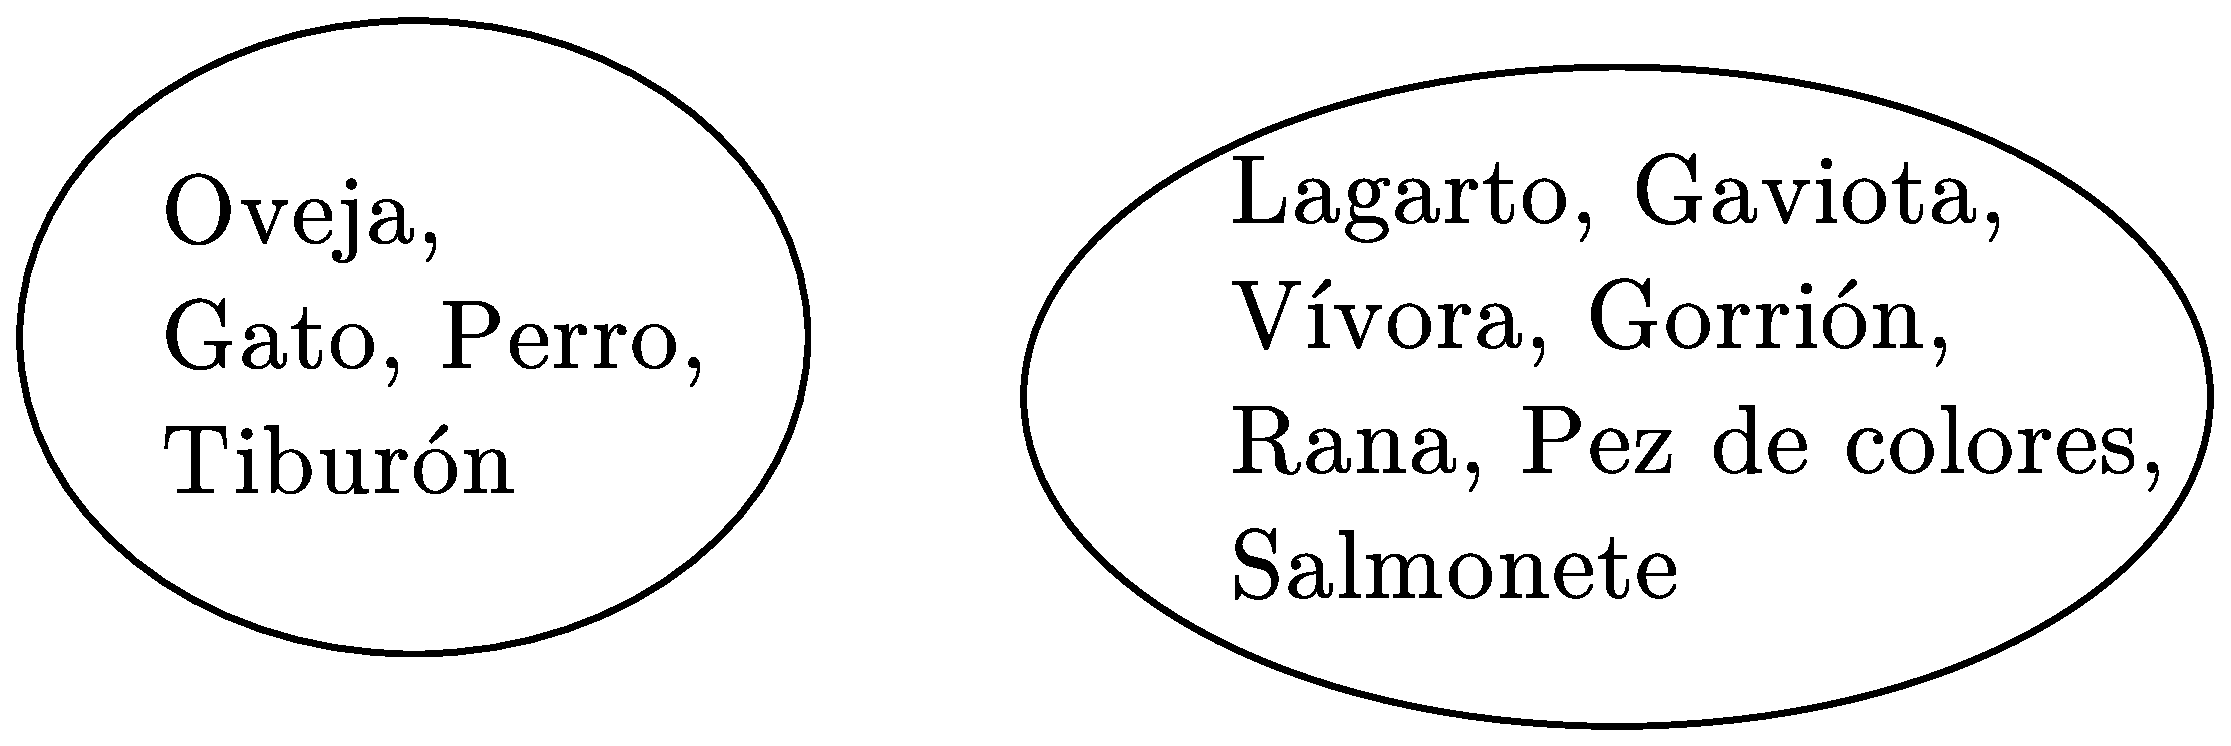
\includegraphics[scale=0.3]{figures/ejemplo1.eps}
\caption{Clustering usando como criterio la manera que llevan a cabo su descendencia}
\label{fig:ejemplo1}
\end{figure}

\begin{figure}[htb]
\centering
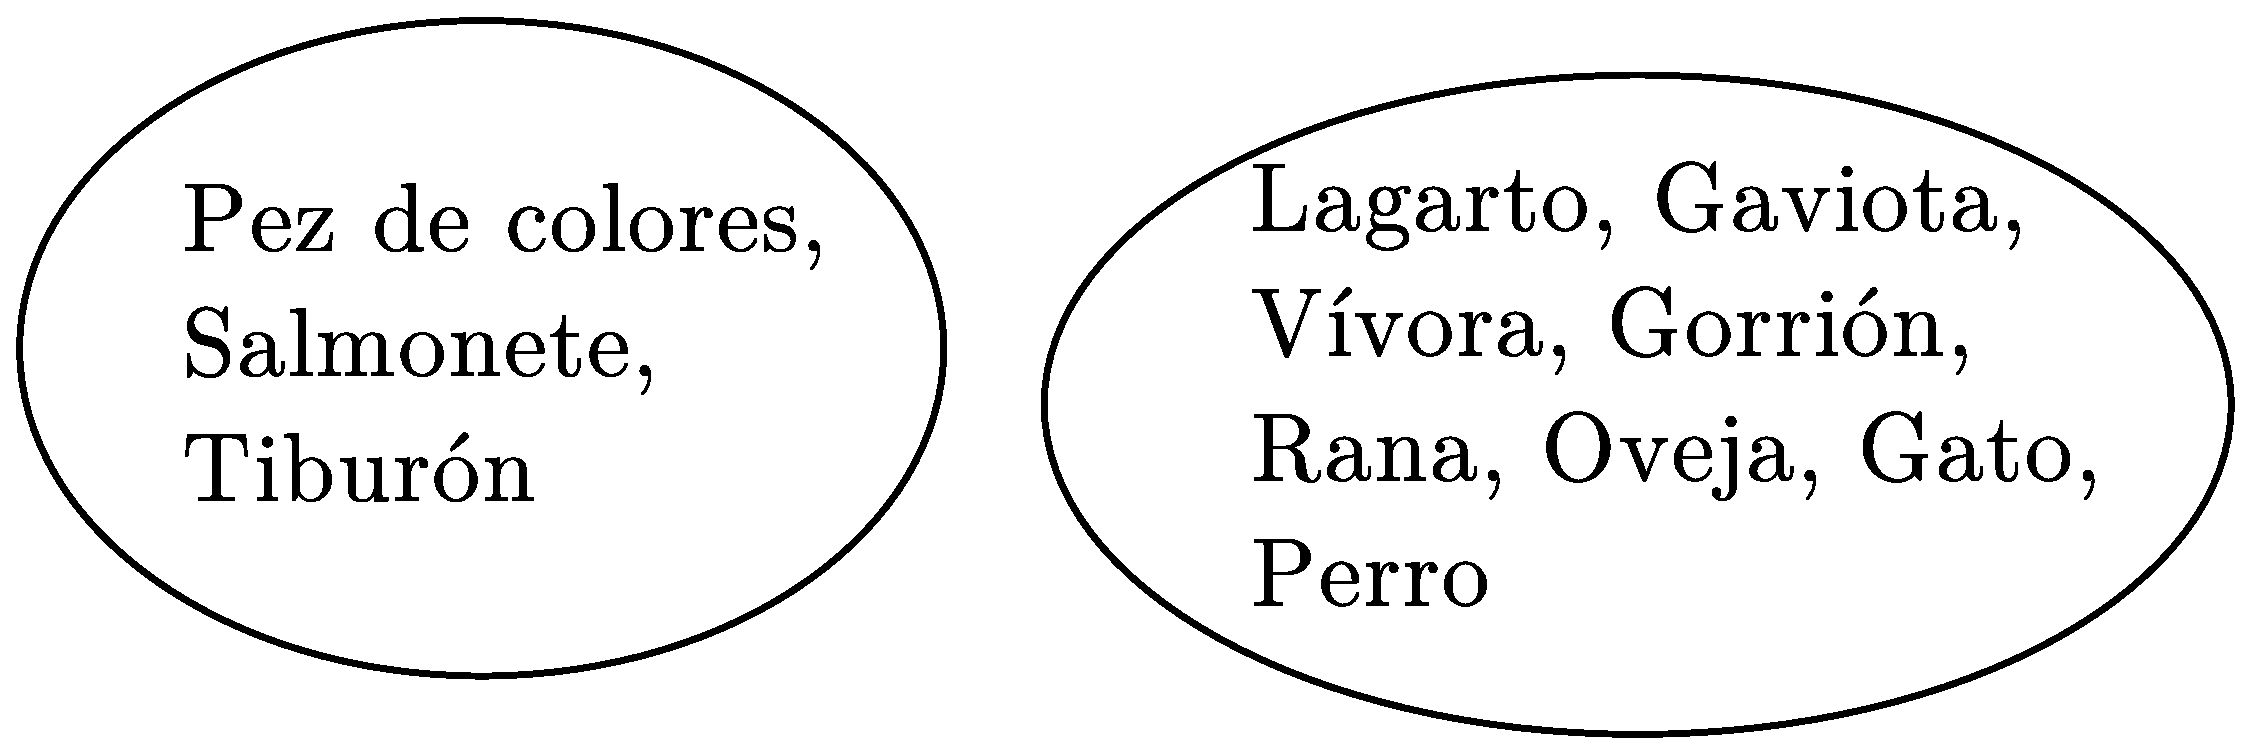
\includegraphics[scale=0.3]{figures/ejemplo2.eps}
\caption{Clustering usando como criterio la existencia de pulmones}
\label{fig:ejemplo2}
\end{figure}

\begin{figure}[htb]
\centering
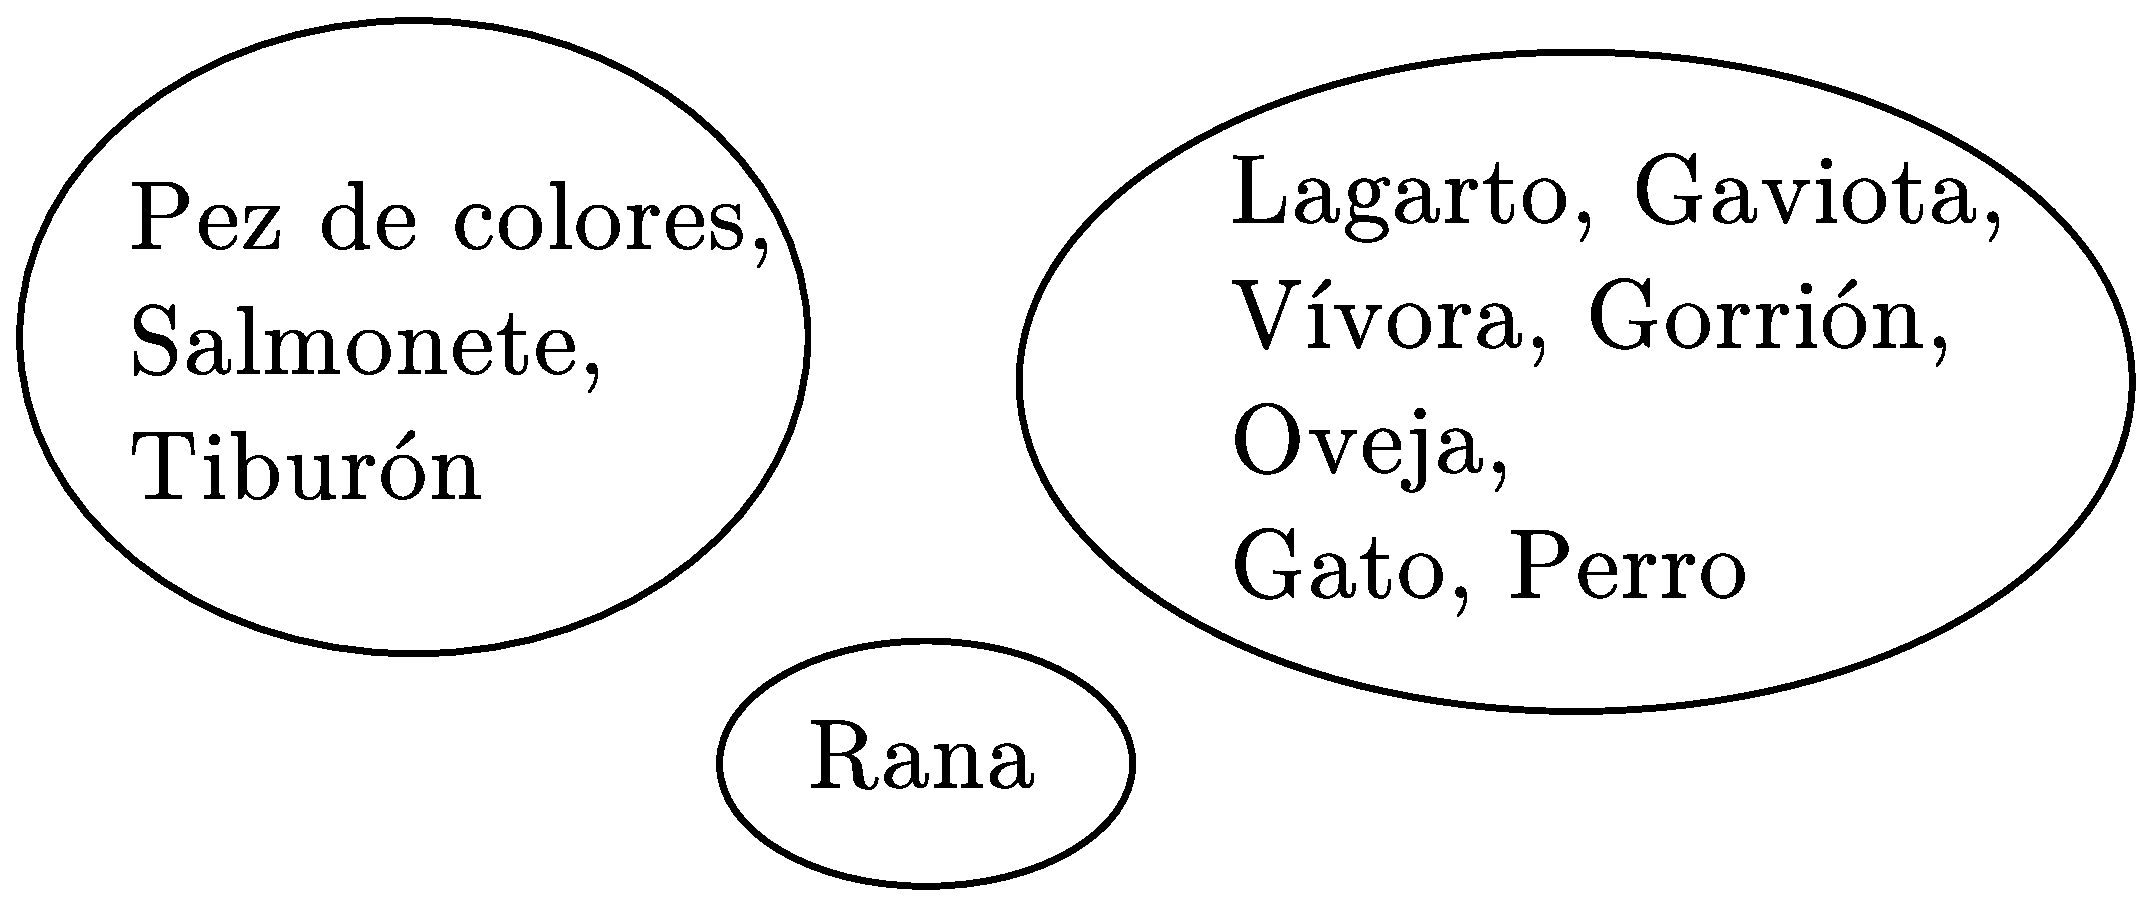
\includegraphics[scale=0.3]{figures/ejemplo3.eps}
\caption{Clustering usado como criterio el ambiente donde viven}
\label{fig:ejemplo3}
\end{figure}

Se puede ver que gracias a la falta de un criterio universal para el clustering,
 \'esta es muy subjetiva en muchos casos.

\item Se puede ver desde el punto de vista de aprendizaje autom\'atico, donde los clusters
correponden a patrones escondidos en los datos, la b\'usqueda de clusters 
es una especie de aprendizaje no supervisado, y el sistema resultante representa
un concepto de datos. Es importante entender la diferencia
entre clustering (aprendizaje no supervisado) y clasificaci\'on supervisada 
(an\'alisis discriminante). En esta \'ultima, se provee una colecci\'on patrones etiquetados
(preclasificados); el problema es etiquetar a un patr\'on recien encontrado, a\'un no etiquetado. 
Tipicamente, los patrones etiquetados (entrenamiento) ya dados son usados para obtener
la descripciones de las clases, que a su vez se utilizan para etiquetar un nuevo patr\'on.
En este caso de clustering, el problema consiste en agrupar una colecci\'on de patrones no etiquetados
en clusters significativos. En este sentidos, las etiquetas se asocian con los clusters tambi\'en,
pero esta categor\'ia de etiquetas son basados en datos, es decir, que se obtienen unicamente
de \'estos.

\item Un algoritmos de clustering se espera que descubra el agrupamiento natural
(pertinente a la noci\'on de los humanos clustering) que existe en una conjunto 
de patrones o puntos de datos. Cada patr\'on puede ser identificado como un punto en un hiperespacio,
llamado espacio de caracter\'isticas, abarcado por las caracter\'isticas asociadas a \'el. La entrada
es un conjunto esos puntos en el espacio carater\'istico multidimensional. Un algoritmo ideal de 
clustering preciso debe presentar como su salida, la etiqueda para cada patr\'on, es decir,
el cluster a cual pertenece cada punto.

\end{itemize}

\'Este problema a sido abordado por diversos campos del conocimiento como la estad\'istica
(an\'aslisis multivariado), teor\'ia de grafos, computaci\'on evolutiva, redes neurales y
as\'i sucesivamente\cite{SwAjAm2009}. Entre sus aplicaciones se encuentra la miner\'ia de datos, expresi\'on de los genes, 
segmentaciones de clientes y procesamiento de im\'agenes, muchas otras. \cite{GaChJi2007}

En especial llama la atenci\'on el \'ultimo mencionado. El procesamiento de im\'agenes es fundamental para los
humanos. Su importancia radica en que la salida puede ser usada como la entrada para 
un modelo basado en sistemas de reconocimiento de objetos.
\'Esto le da una gama de aplicaciones gigantescas: cualquier tipo de reconicimiento de im\'agenes.
Tambi\'en en el \'area m\'edica puede ayudar a encontrar regiones en las im\'agenes que sean tumores,
que posiblemente humano no logre identificar, lo que es extremadamente
\'util.

Brucker en \cite{Br1978} ilustr\'o que el problema es NP-hard cuando el n\'umero 
de clusters excede 3.

\subsection{Definici\'on} \label{sect:dclustdef} \label{sect:dclustd}

Siguiendo con \cite{SwAjAm2009} antes de dar un definici\'on matem\'atica al problema hay que hablar de 
los siguientes t\'erminos que van a ser usados a trav\'es de la tesis:

\begin{itemize}

\item {\bf Patr\'on o vector caracter\'istico:} Se va a encargar de abstraer matem\'aticamente las
caracter\'isticas que poseen los objetos a los cuales se les har\'a el clustering.

\item {\bf Caracter\'istica:} Es una componente de un patr\'on. \'Esta representa
la base usada para clasificaci\'on de los patrones.

\item {\bf Cluster:} Es un grupo de patrones similares, y los patrones de dos clusters 
distintos no deben ser similares.

\item {\bf Hard clustering:} Cada patr\'on se asigna solamente a un cluster.

\item {\bf Medici\'on de distancia:} Es la m\'etrica con la cual se va a evaluar
la disimilaridad entre los patrones. M\'as adelante se habl\'a en m\'as detalle.

\end{itemize}

Ahora se puede dar una definici\'on formal al problema:

Sea $P = \{ P_1, P_2, \dots , P_N\}$ un conjunto de N patrones, 
donde cada uno tiene M caracter\'isticas. Éstos pueden
ser reprentados por una matriz $Z_{NxM}$. El vector de la fila $i$ caracteriza al 
patr\'on $i$ del conjunto $P$ y cada elemento $Z_{i,j}$ en $Z_i$ su caracter\'istica $j$.
Dada tal matriz Z$_{NxM}$ la idea es que un algoritmo de clustering intente hallar
el particionamiento $C = \{ C_1, C_2, \dots , C_K \}$ tal que los patrones
en el mismo cluster $C_i$ su similaridad sea la mayor y entre clusteres diferentes
sean lo más disimilar:

\begin{enumerate}

\item Cada cluster debe tener por lo menos un patr\'on asignado:

$\forall i | i \in \{1, 2, \dots, K\} : C_i \neq \emptyset$

\item Dos patrones distintos no tienen ning\'un patr\'on en com\'un:

$\forall i,j | i,j\in \{1, 2, \dots, K\} \land i \neq j:  C_i \cap C_j \neq \emptyset$

\item Cada patr\'on debe estar asignado a un cluster:

$\bigcup_{i=1}^{K} C_i = P$

\end{enumerate}

Dado que el conjunto de datos dados puede ser partidionado de varias maneras
manteniendo las propiedades de arriba, es necesaria una función objetico o en otras palabras
una medida de que tan buena es la partici\'on. El problema se comvierte en hallar
una partici\'on $C^*$  \'optima o lo m\'as cercano a ella en comparaci\'on a 
las otras soluciones posible $C = \{ C^1, C^2, \dots, C^{T(N,K)} \}$ donde 
$T(N,K) = { {1 \over K!} \times {\sum_{i=1}^{K} (-1)^i  \binom{K}{i} (K-i)^i} }$
es el n\'umero de particiones posibles. \'Esto es lo mismo que optimizar $f(Z_{NxM}, PC)$,
donde PC es un partici\'on del conjunto C y $f$ es una funci\'on objetivo que
cuantifica la calidad del particionamiento en base a la similaridad o disimilaridad
de los patrones.

\section{M\'etricas de distancia} \label{sect:mdist}

En  \cite{SwAjAm2009} explican que comunmente hay dos tipos: la que mide la disimilaridad y el caso contrario (la
similaridad). La primero es mas grande a medida que dos patrones son
m\'as diferentes. La segunda es justamente el opuesto, es m\'as
grande a medida que los patrones se parecen m\'as.

Entre las de disimilaridad las m\'as populares donde la distancia euclideana entre
dos vectores $Z_i$ y $Z_v$ es la siguiente:

\[
d(Z_u,Z_v) = \sqrt {\sum_{i=1}^M {(Z_{u,i} - Z_{v,i})}^2} = \parallel Z_u - Z_v \parallel
\]

\'Esta no es mas que un caso especial para ($\alpha = 2$) de la m\'etrica de 
Minkowski, definida como:

\[
d^{\alpha}(Z_u,Z_v) = \sum_{i=1}^M {(Z_{u,i} - Z_{v,i})}^{1 \over \alpha} = \parallel Z_u - Z_v \parallel ^ {1 \over \alpha}
\]

Cuando $\alpha = 1$ se conoce como la distancia Manhattan. Otra bastante com\'un es
la de la distancia del coseno, que es lo siguiente:

\[
Z_u . Z_v =  {{\sum_{i=1}^M {Z_{u,i} . Z_{v,i}}}  \over { \parallel Z_u \parallel \parallel Z_v \parallel}}
\]

\section{Funci\'on objetivo} \label{sect:fobjetivo}

\'Esta se va a encargar de medir la calidad de una soluci\'on por ello
debe medir dos cosas: cohesi\'on, es decir, los patrones en el mismo clusters
deben ser similares, y separaci\'on, que significa que los clusters
deben estar bien separados.

Dos de los m\'as comunes como explica \cite{SwAjAm2009} son:

\begin{itemize}

\item {\bf Davis-Bouldin:}

Esta medida es la la propoci\'on de la suma intra-cluster entre
la separaci\'on entre los clusters, y use tanto los clusters como sus medias. Se tiene:

\[
S_{i,r} = {[{ { {1} \over {N_i}} {\sum_{Z \in C_i} { \parallel Z - m_i \parallel }_2^r}} ]^{1 \over r}}
\]

\[
d_{ij,t} = \{ \sum_{p=1}^M |m_{i,p} - m_{j,p}|^t \} ^{1 \over t} = \parallel m_i - m_j \parallel_t
\]

donde $m_i$ es el centroide del cluster $i$, $r$ y $t$ son enteros y pueden ser elegidos
independientemente, $N_i$ es el numero de objetos en el $i$-\'esimo cluster $C_i$.

\[
R_{i,rt} = {max_{j \in K, j \neq i} \{ {{S_{i,r} + S_{j,r}} \over {d_{ij,t}}} \}}
\]

Finalmente:

\[
DB(K) = {1 \over K} \sum_{i=1}^K R_{i,rt}
\]

\item {\bf Medida CS:} Es bantante parecido al DB y se calcula de la siguiente manera:

\[
CS(K) = {{\sum_{i=1}^K [{ 1 \over |C_i|} \sum_{Z_p \in C_i} max_{Z_y \in C_i} \{ d(Z_p,Z_y) \} ]} \over {\sum_{i=1}^K [min_{j \in K, j \neq i} \{ d(m_i, n_j) \}]}}
\]

\'Esta es mucho mas eficiente atacando clusters con diferentes densidad y/o tama\~nos,
pero es muy costosa en t\'ermino de carga computacional.

\end{itemize}

Otra es la que explica \cite{OmEnSa2005} es que en el contexto de 
clustering de datos, una partícula o indivuduo representa
los $K$ centroides de los clusters. Así que cada partícula $x_i$ es
construída como $x_i = (m_{i,1}, ..., m_{i,k}, ..., m_{i,K})$ donde
$m_{i,k}$ se refiere al centroide del $k$-ésimo cluster. La calidad
de cada uno es medida usando:

\[
f(x_i,Z_i) = w_1 \overline{d}_{Max}(Z_i,x_i) + w_2 (z_{Max} - d_{Min}(x_i)) + w_3 J_{e,i}
\]

donde $z_{Max}$ es el máximo valor del conjunto de datos (en el contexto
de imágenes digitales $z_{Max} = 2^s - 1$ para una imagen de $s$-bits);
$Z_i$ es la matriz representando la asignación de patrones a los clusters
de la partícula $i$. Las constantes $w_1$, $w_2$ y $w_3$ son definidas por el usuario
usadas para determinar la contribución de cada uno de los sub-objetivos.
También:

\[
\overline{d}_{Max}(Z_i,x_i) = \max_{1 \leq k \leq K} \left[ \displaystyle\sum_{\forall z_p \in C_{i,k}} d(z_p,m_{i,k})/n_{i,k}\right]
\]

es la máxima distancia Euclediana promedio de las partículas en sus
clusters asociados.

\[
\overline{d}_{Min}(x_i) = \min_{\forall k, l, k \neq l} \left[ d(m_{i,k},m_{i,l})\right]
\]

es la distancia Euclediana mínima entre un par de clusters.

Y:

\[
J_e = \cfrac{\displaystyle\sum_{k = 1}^K \left[ \displaystyle\sum_{\forall Z_p \in C_k} d(Z_p, m_k) \right] / n_k}{K}
\]

es la cuantificación del error, donde $C_k$ es el $k$-ésimo cluster y $n_k$ es el número de pixeles
en $C_k$.


\section{K-means} \label{sect:kmeans}

Es uno de los algoritmos m\'as usados para atacar el problema de clustering.
Fue dise\~na do para datos num\'ericos en donde cada cluster tiene un centro llamado
media (mean). Este tiene un n\'umero $K$ de clusters ya establecidos. Funciona
del siguiente modo: para unos $K$ clusters ya inicializados, va a ir tomando 
un objeto, luego buscar si su distancia con respecto a la media de otro
cluster es menor a la del suyo, cambiarlo y recalcular las medias. \'Este
ciclo va a ir ejecutantodose hasta que cierta condici\'on de parada se cumpla.\cite{GePo2010}

La media, tambi\'en llamada centroide,  de un cluster $C_i$ (con $1 \leq i \leq K$)
se define del siguiente modo:

\[
{1 \over |C_{i}|} \sum_{v \in C_{i}} v
\]

El pseudoc\'odigo es el siguiente:

\begin{lstlisting}[mathescape, language=Pascal]
  Incialización.
  Mientras no se cumpla el criterio de parada.
    Tomar $i$ de un cluster.
    Buscar un clusjer j tal que d(i,media de j) sea la menor entre todos los clusters.
    Cambiar $i$ al cluster $j$.
    Recalcular los centroides.
\end{lstlisting}

La inicializaci\'on puede ser aleatoria o bien mediante un m\'etodo m\'as
sofiticado como un algoritmo greedy.

Sus propiedades m\'as importantes son las siguientes:

\begin{itemize}

\item Es bastante eficiente para hacer clustering de grandes conjuntos de datos,
ya que su complejidad es lineal al n\'umero de datos $O(N)$.

\item Tiende a quedarse en \'optimos locales.

\item S\'olo sirve en datos num\'ericos.

\item Su buen funcionamiento depende de la inicializaci\'on de los clusters.

\end{itemize}

\section{Metaheur\'isticas} \label{sect:meta}

\subsection{Abeja} \label{sect:metabee}

\subsection{Gen\'etico} \label{sect:metaga}

Imita la evoluci\'on gen\'etica de las especias. Un aspecto importante es que
explora varias soluciones a la vez, y no se enfoca en s\'olo una. A medida que
se ejecuta, las soluciones, tambi\'en llamadas individuos o cromosomas, 
toman parte en un proceso reporoductivo, donde interactuan, mezclan y producen
hijos que retiene algunas caracter\'isticas de sus padres. \'Este proceso
que conlleva a la creaci\'on de nuevas soluciones (hijos) esta basada en
la selecci\'on, cruce y mutaci\'on\cite{DoGeGr2007}.

Los cromosomas se pueden codificarse de bastantes modos, donde el m\'as 
com\'un es mediante strings de n\'umeros binarios (100101110101).

En el clustering exiten los siguientes, tal como explica \cite{HrCaFr2009}:

\begin{itemize}

\item {\bf Binar\'ia:} Es un string de logitud $N$, donde en cada posici\'on
corresponde a un objeto en particular. El valor es 1 o 0 dependiendo si 
el objeto es un centroide o no.

{\bf Entera:}

Es posible las siguientes dos:

\begin{itemize}

\item Por etiqueta: Se tiene un arreglo de tama\~no $N$ donde en cada posici\'on
se coloca el cluster al cual pertenece el objeto.

El problema de \'esta recae en que se pueden repetir muchas veces una soluci\'on ($K!$ maneras cada una).

\item Por centroides: Si se tienen $K$ clusters se usa un arreglo de este tama\~no
indicando cual es el centroide de cada clusters.

\end{itemize}

{\bf Real:} Sirve para representar las coordenadas de los centroides de los clusters.
Su longitud va a ser $K \times M$.

\end{itemize}

El pseudoc\'odigo es de la siguiente manera (hay m\'as interpretaciones posibles):

\begin{lstlisting}[mathescape, language=Pascal]
  Inicialización.
  Mientras no se cumpla el criterio de parada.
    Si rand(0,1) <= pc
      Selección.
      Cruce.
      Si rand(0,1) <= pm
        Mutación.
      Si los hijos tiene mejor función objetico que los papas.
        Colocarlos en la población y eliminar a los padres.
\end{lstlisting}

Donde pc es la probabilidad de cruce, pm la de mutaci\'on y rand(0,1)
es una funci\'on que devuelve un n\'umero aleatorio entre 0 y 1. Y el resto
se define como :

\begin{itemize}

\item {\bf Inicializaci\'on:} Los par\'ametros son fijados y se
crean los cromosomas de la poblaci\'on.

\item {\bf Selecci\'on:} Consiste en elegir los padres. 

En \cite{GePo2010} comentan sus formas de implementar m\'as comunes:

\begin{itemize}

\item Tomar m\'as cuenta los individuos
con mejor funci\'on objetvo. Para ello se puede usar el m\'etodo bastante conocido
llamado roulette-wheel. 

\item Selecci\'on por torneo, en
donde un conjunto de cromosomas $\tau$ son elegisdos y comparados, los mejores
son elegidos para ser padres. 

Una de sus ventajas es que s\'olo necesita un orden de preferencia entre pares,
y puede por lo tanto hacer frente a situaciones en las que no hay ninguna función objetivo formal,
es decir puede tratar con casos donde la funci\'on objetivo es muy subjetiva.

\end{itemize}

\item {\bf Cruce:}

Consiste en replazar los genes de uno de los padres por los del otro. Se puede hacer
de la siguiente manera continuando \cite{GePo2010}:

\begin{itemize}

\item {\bf De un punto:} Si se tienen dos padres de longitud $X$, se va a tomar
un punto entre $[1,X-1]$ y se generan dos hijos de la siguiente manera: el primero,
de 0 al punto con los genes del primer padre y del punto a $X$, y el segundo es 
lo contrario.

Si se tienen los padres [1 3 2 4 6]  y [5 1 3 6 2] y el punto 
de crude es el 2, entonces se generan los siguientes hijos:

[1 3 3 6 2] y [5 1 2 4 6]

\item {\bf De dos punto:} Ac\'a se eligen dos puntos distintos que cumplan con la 
misma condici\'on como en el de un punto. Para explicar es mucho mas sencillo
mediante un ejemplo:

Si se tienen los padres [1 3 2 4 6]  y [5 1 3 6 2] y los puntos 
de crude son el 2 y 4, entonces se generan los siguientes hijos:

[1 3 3 6 6] y [5 1 2 6 2]

De esta misma forma se puede extender para m\'as puntos.

\end{itemize}

\item {\bf Mutaci\'on:}

Consiste en modificar uno de los cromosomas bien sea de la poblaci\'on
o uno de los hijos generados. Un caso bastante com\'un es el de usar una m\'ascara
cuando los cromosomas son binarios\cite{GePo2010}.

Por su lado en esa misma referencia se comenta que para clustering se pueden usar los siguientes:

\begin{itemize}

\item En el caso que se use la representaci\'on binaria, alternar los bits es un
buen operador.

\item Cuando la representaci\'on es de enteros de etiquedas, se puede cambiar
el cluster al cual pertenece uno de los objetos.

\item Remplazar uno de los centroides por uno de los objetos pertenecientes a ese
cluster.

\end{itemize}

\end{itemize}

\subsection{DE} \label{sect:metade}

Es un algoritmo basado en poblaci\'on de
optimizaci\'on global que hace uso de una representaci\'on de punto flotante
(codificaci\'on real), bastante parecido al gen\'etico. Se tienen los pasos de cruce 
y selecci\'on, pero no mutaci\'on. Su funcionamiento seg\'un \cite{SwAjAm2008}
es el siguiente:

El $i$-\'esimo vector individual (cromosoma)
de la poblaci\'on con tiempo (generaci\'on) $t$ tiene $d$ componentes
dimensiones:

%Ejemplo de vector.
%INICIO
\begin{center}
$ \overrightarrow{Z_i}(t) = [ Z_{i,1}(t), Z_{i,2}, \cdots, Z_{i,d}(t) ] $
\end{center}
%END

Para cada vector individual $\overrightarrow{Z_k}(t)$ que pertenece
a la poblaci\'on actual, el DE aleatoriamente toma tres individuos
$\overrightarrow{Z_i}(t)$, $\overrightarrow{Z_j}(t)$ y $\overrightarrow{Z_m}(t)$ de la misma generaci\'on (de modo que sean distintos $k$, 
$i$, $j$ y $m$). Entonces calcula la diferencia entre $\overrightarrow{Z_i}(t)$ y $\overrightarrow{Z_j}(t)$, lo escala por un escalar $F$
(usualmente $F \in [0, 1]$) y crea un hijo prueba $\overrightarrow{U_i}(t + 1)$ a\~nadiendo el resultado a $\overrightarrow{Z_m}(t)$. De modo
que para la $n$-\'esima componente del vector:

\[
  U_{k,n}(t+1) =
  \begin{cases}
    Z_{m,n}(t) + F(Z_{i,n}(t) - Z_{j,n}(t))  & \text{si } rand_n(0,1) < Cr\\
    Z_{k,n}(t)                               & \text{sino}
  \end{cases}
\]

Donde $Cr \in [0, 1]$ es un escalar que es par\'ametro de el algoritmo,
llamado la \emph{tasa de cruce}. Si el nuevo hijo tiene mejor valor
con la funci\'on objetivo, entonces reemplaza al padre en la siguiente
generaci\'on, sino, el padre entonces se queda en la misma:
\[
  \overrightarrow{Z_i}(t+1) =
  \begin{cases}
    \overrightarrow{U_i}(t+1) & \text{si } f(\overrightarrow{U_i}(t+1)) > f(\overrightarrow{Z_i}(t)) \\
    \overrightarrow{Z_i}(t)   & \text{si } f(\overrightarrow{U_i}(t+1)) \leq f(\overrightarrow{Z_i}(t))
  \end{cases}
\]
donde $f$ es la funci\'on objetivo a ser maximizada.

\subsection{PSO} \label{sect:metapso}

\subsection{Hormiga} \label{sect:metaant}

Hormiga es una metaheurística usada para resolver problemas combinatorios
difíciles. \'Esta se inspira en los diversos comportamientos de las hormigas.
Comunmente se basa en el rastro de feromona y el comportamiento de seguirlo 
de éstas, usado en la búsqueda de comida. Una hormiga que se est\'a moviendo 
suelta feromonas en el suelo, as\'i marcando un camino. \'Este químico, que 
desaparece con el tiempo, el reforzado si otras hormigas usan ese mismo camino.
Por lo tanto, las mejores v\'ias incrementan su nivel de feromonas con el tiempo, 
y al contrario con los peores. Fue propuesto por Marco Dorigo en 1992, 
y lo ha expandidos en sus trabajos posteriores.
\cite{GePo2010} \cite{Le2007}

Su funcionamiento como explica \cite{GePo2010} es el siguiente: primero, $m$ hormigas contruyen
soluciones del problema, sesgada por la informaci\'on de las feromonas y posiblemente
por las disponible por parte de las heur\'isticas. Una vez que las hormigas hallan completado
sus soluciones, se pueden mejorar mediante una b\'usqueda local. Finalmente,
antes de empezar con la siguiente iteraci\'on , los ratros de feromonas son
actualizados para reflejar la experiencia de b\'usqueda de las hormigas:

\begin{lstlisting}[mathescape, language=Pascal]
  Incialización.
  Mientras no se cumpla el criterio de parada.
    Construcción de las soluciones.
    Aplicar búsqueda local.
    Actualizar feromonas.
\end{lstlisting}

\begin{itemize}

\item {\bf Inicializaci\'on:} Los par\'ametros son establecidos y todas las variables 
de feromonas son puestas en t$_{0}$, el cual es un par\'ametro del algoritmo.

\item {\bf Construcci\'on de las soluciones:} Cada hormiga empieza con una soluci\'on vac\'ia
$s_p = \emptyset $. En cada paso de las construcci\'on , una hormiga
extiende su soluci\'on parcial actual $s_p$ eligiendo un posible componente $c_i^j \in N(s_p) \subseteq C$ 
y agregandolo a \'esta. $N(s_p)$ es el conjunto de los
componentes de soluci\'on que pueden ser agregados manteniendo su validez
y es definido implicitamente por el proceso de construcci\'on de soliciones
que las hormigas implementan. 

La elecci\'on del componente de la soluci\'on que se quiere agregar es 
hecha probabil\'isticamente en cada paso de la construcci\'on. La manera m\'as
com\'un es la siguiente:

\[
p(c_i^j) = {\tau_{ij}^{\alpha}  \times [ \eta (c_i^j) ]^{\beta}}  \over { \sum_{c_i^l \in N(s_p)} \tau_{il}^{\alpha} \times [\eta (c_i^l)]^{\beta}] } 
\]

donde $\eta(.)$ es una funci\'on  que asigna a cada posible componente 
de la soluci\'on $c_i^j \in N(s_p)$ un valor heur\'istico, que es usualmente
llamada infomaci\'on heur\'istica. Los par\'ametos $\alpha$ y $\beta$ 
determinan la relativa influencia de los rastros de feromonas e informaci\'on
heur\'istica, por lo tanto influyendo significativamente en el comportamiento
del algoritmo.


\item {\bf Aplicar b\'usqueda local:} Una vez obtenidas las soluciones candidatos,
estas puede ser mejoradas aplicando algoritmos de b\'usqueda local.

\item {\bf Actualizaci\'on de las feromonas:}: tiene como objetivo
hacer que los compentes de una buena soluci\'on, 
sean m\'as deseables para las hormigas en las siguientes iteraciones. Hay esencialemente
dos mecanismos para lograr este objetico. El primero es el dep\'osito de feromonas,
el cual incrementa el nivel de feromonas de los coponentes de una soluci\'on
que est\'an asociados con un conjunto selccionado $S_{upd}$ de buenas soluciones.
El segundo es la evaporaci\'on del rastro de feromonas, el cual es un mecanismo
que decrece a medida que el tiempo pasa el dep\'osito de feromonas. Desde el punto de
vista pr\'actico, \'este es necesario para evitar la r\'apida convergencia del algoritmo
en una regi\'on sub\'optima. Es comunmente implementada de la siguiente
manera:

\[
\tau_{ij} = (1-\rho)\tau_{ij} + \sum_{s \in S_{upd} \land c_i^j \in s} g(s)
\]

donde $S_{upd}$ es el conjunto de soluciones usadas para depositar feromonas, 
$\rho in (0,1]$ es un par\'ametro llamada constante de evaporaci\'on,
$g(.):S \rightarrow  \Re^+$ es una funci\'on que determina la calidad
de la soluci\'on.
\end{itemize}

Adem\'as en \cite{OuBa2007} exponen que actualmente los cient\'ificos est\'an 
empezando a inspirarse en la manera que las hormigas crean sus cementerios: limpian sus nidos
y crean pilas de cad\'averes. 
Tambi\'en de la organizaci\'on de cr\'ias, donde son agrupadas
de acuerdo a su tama\~no. El principio recae en la atracci\'on
entre los objetos transportados. Los clusters pequeños de objetos
similares van creaciendo atrayendo a las hormigas a despositar m\'as
objetos de acuerdo con su tama\~no o tipo. Este feedback positivo
conlleva a la formaci\'on de clusters homog\'enos.

El pioner en este trabajo es Deneubourg et al., donde aplican el
m\'etodo para tareas en rob\'otica. Este ha sido modificado por Lumer
y Faita para extenderlo a an\'alisis num\'erico de datos.
En estos algoritmos los datos son dispersados aleatoriamente
en un grid de dos dimensiones. Cada hormiga se mueve aleatoriamente
dentro de \'este agarrando y soltando estos datos. La decisi\'on
de agarrar o soltar un dato es aleatoria,
pero es influenciada por los datos en el vecindario, 
causando que datos similares tengan m\'as probabilidad de
estar juntos. La probabilidad de soltar un dato incrementa
en zonas de mayor densiadad de datos similares, y decrementa
cuando sucede el contrario.  En contraste
la probabilidad de agarrar un dato incrementa en las zonas de
menor densidad y decrementa en el opuesto.
\'Esta est\'an dadas por:

\[
P_p(i) = {k_1 \over {k_1 + f(i)}}
\]

\[
P_d(i) = 
  \begin{cases}
    2f(i) & \quad \text{si $f(i)<k_2$}\\
    1     & \quad \text{si $f(i) < k_2s$}\\
  \end{cases}
\]

\[
f(i) =
  \begin{cases}
    {{1} \over {s^2}} \sum_{j \in R(r(i))} {{1 - {d(i,j)}} \over \alpha} & \quad \text{si $f > 0$}\\
    0     & \quad \text{sino}
  \end{cases} 
\]

Donde $r(i)$ es la posici\'on del dato $i$ dado en el grid y $f(i)$ es una medida
del promedio de disimilaridad del dato $i$ con respecto a los otros $j$
presentes en su vencindario $R$ con tama\~no $s \times s$. $\alpha$
es la escala de disimilaridad y es clave en la ejecuci\'on del algoritmo:

\[
\alpha = {{1 \over {N(N-1)}} \sum_{i=1}^N \sum_{j=1}^N d(p_i,p_j)}
\]

El n\'umero de aplicaciones es bastante grande: resolver problemas
desde data clustering, programaci\'on (scheduling), balanceo
de l\'inea de equilibrio, TSP probabil\'istico, secuenciaci\'on de 
ADN, etc. \cite{GePo2010}
